\documentclass[crop,tikz]{standalone} 
\usepackage{tikz, amsmath, amssymb, graphicx} 

\usetikzlibrary{positioning, shapes.geometric} 

\begin{document} 

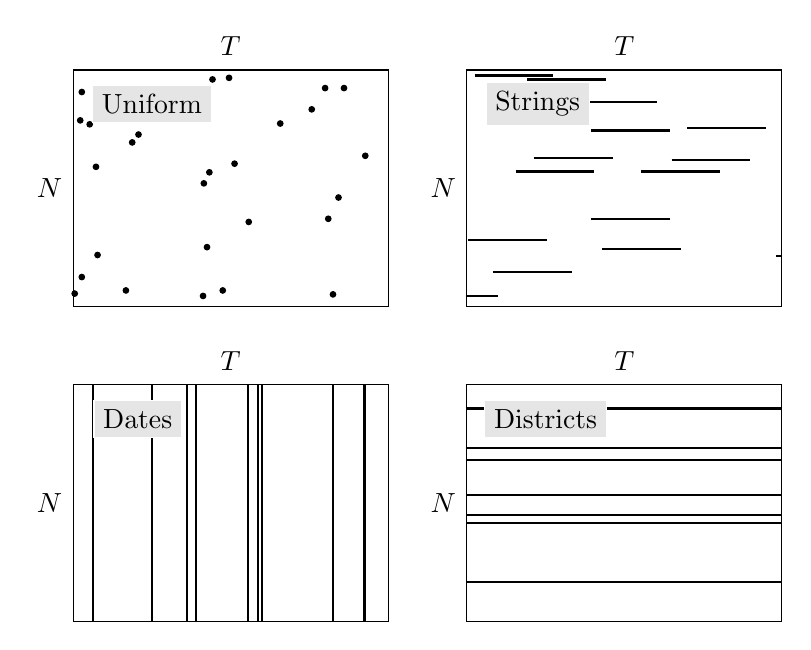
\begin{tikzpicture}

\draw[draw=black] (0, 0) rectangle ++(4, 3);

\draw (-0.3, 1.5) node {$N$};
\draw (2, 3.3) node {$T$};

\draw (4.7, 1.5) node {$N$};
\draw (7, 3.3) node {$T$};

\draw (4.7, -2.5) node {$N$};
\draw (7, -0.7) node {$T$};

\draw (-0.3, -2.5) node {$N$};
\draw (2, -0.7) node {$T$};

% \draw [-stealth](0.6,3.28) -- (1.3,3.28);
% \draw [-stealth](-0.3,2.3) -- (-0.3,1.6);

% \draw (2,3.5) node {Uniform};
% \draw (1,2.5) node {Uniform};





\filldraw[black] (1.70,0.75) circle (1pt);
\filldraw[black] (0.21,2.31) circle (1pt);
\filldraw[black] (0.39,2.37) circle (1pt);
\filldraw[black] (1.66,1.56) circle (1pt);
\filldraw[black] (0.31,0.65) circle (1pt);
\filldraw[black] (3.30,0.15) circle (1pt);
\filldraw[black] (0.67,0.20) circle (1pt);
\filldraw[black] (0.75,2.08) circle (1pt);
\filldraw[black] (1.77,2.88) circle (1pt);
\filldraw[black] (0.11,2.72) circle (1pt);
\filldraw[black] (2.05,1.81) circle (1pt);
\filldraw[black] (0.29,1.77) circle (1pt);
\filldraw[black] (0.02,0.16) circle (1pt);
\filldraw[black] (1.73,1.70) circle (1pt);
\filldraw[black] (3.03,2.50) circle (1pt);
\filldraw[black] (0.83,2.18) circle (1pt);
\filldraw[black] (3.71,1.91) circle (1pt);
\filldraw[black] (0.11,0.37) circle (1pt);
\filldraw[black] (0.61,2.59) circle (1pt);
\filldraw[black] (3.20,2.77) circle (1pt);
\filldraw[black] (2.23,1.07) circle (1pt);
\filldraw[black] (2.63,2.32) circle (1pt);
\filldraw[black] (3.24,1.11) circle (1pt);
\filldraw[black] (1.98,2.90) circle (1pt);
\filldraw[black] (1.90,0.20) circle (1pt);
\filldraw[black] (3.44,2.77) circle (1pt);
\filldraw[black] (1.65,0.13) circle (1pt);
\filldraw[black] (0.09,2.36) circle (1pt);
\filldraw[black] (3.37,1.38) circle (1pt);
\filldraw[black] (0.38,2.77) circle (1pt);

\draw[draw=black] (5, 0) rectangle ++(4, 3);


\draw[thick] (5.77,2.88) -- (6.77,2.88);
\draw[thick] (6.72,0.73) -- (7.72,0.73);
\draw[thick] (5.62,1.71) -- (6.62,1.71);
\draw[thick] (7.80,2.26) -- (8.80,2.26);
\draw[thick] (8.93,0.64) -- (9.00,0.64);
\draw[thick] (6.58,1.11) -- (7.58,1.11);
\draw[thick] (5.33,0.43) -- (6.33,0.43);
\draw[thick] (6.58,2.23) -- (7.58,2.23);
\draw[thick] (5.02,0.84) -- (6.02,0.84);
\draw[thick] (6.41,2.59) -- (7.41,2.59);
\draw[thick] (5.85,1.88) -- (6.85,1.88);
\draw[thick] (5.00,0.13) -- (5.39,0.13);
\draw[thick] (7.21,1.71) -- (8.21,1.71);
\draw[thick] (7.60,1.86) -- (8.60,1.86);
\draw[thick] (5.10,2.93) -- (6.10,2.93);


\draw[draw=black] (0, -4) rectangle ++(4, 3);

\draw[thick] (1,-4) -- (1,-1);
\draw[thick] (0.25,-4) -- (0.25,-1);
\draw[thick] (1.45,-4) -- (1.45,-1);
\draw[thick] (1.56,-4) -- (1.56,-1);
\draw[thick] (2.22,-4) -- (2.22,-1);
\draw[thick] (2.35,-4) -- (2.35,-1);
\draw[thick] (2.4,-4) -- (2.4,-1);
\draw[thick] (3.3,-4) -- (3.3,-1);
\draw[thick] (3.7,-4) -- (3.7,-1);

\draw[draw=black] (5, -4) rectangle ++(4, 3);

\draw[thick] (5,-1.8) -- (9, -1.8);
\draw[thick] (5,-1.95) -- (9, -1.95);
\draw[thick] (5,-2.4) -- (9, -2.4);
\draw[thick] (5, -1.3) -- (9, -1.3);
\draw[thick] (5, -2.65) -- (9, -2.65);
\draw[thick] (5, -2.75) -- (9, -2.75);
\draw[thick] (5, -3.5) -- (9, -3.5);


\node[rectangle,draw=white,fill = black!10!white] (r) at (1,2.57) {Uniform};
\node[rectangle,draw=white,fill = black!10!white] (r) at (0.82,-1.43) {Dates};
\node[rectangle,draw=white,fill = black!10!white] (r) at (5.9,2.57) {Strings};
\node[rectangle,draw=white,fill = black!10!white] (r) at (6,-1.43) {Districts};


\end{tikzpicture}
\end{document} 
